\documentclass[11pt,a4paper]{report}
\usepackage[utf8]{vietnam}
\usepackage{amsmath}
\usepackage{amssymb}
\usepackage{graphicx}
\begin{document}
	\begin{center}
		\textbf{Tổng quan}
	\end{center}
\textbf{I - Nền tảng}
0. Bảng ghi nhớ logic
1. Tập hợp
2. Quan hệ nhị phân
3. Hàm số
4. Quan hệ nội nhị phân
5. Tính toán và đệ quy
6. Khái niệm phức
\textbf{I - Đồ thị}
7. Dấu chấm và mũi tên
8. Đường dẫn và mạch
9. Đóng cửa bắc cầu
10. Cây và kết nối
11. Đồ thị đa phần
\textbf{Đại số}
12. Toán tử và đại số
13. Monoid và ngôn ngữ
14. Diode và đại số đường đi
15. Đại số Bôle
16. Đại số Kleene và ô tự động các trạng-thái hữu hạn
\part{Cơ bản}
\chapter{Bảng ghi nhớ logic}
Có thể bỏ qua chương này khi đọc lần đầu tiên : nó chỉ mang tính chất hỗ trợ trí nhớ ngắn gọn và chỉ nhằm mục đích xóa bỏ những nghi ngờ nhất định mà người đọc có thể có trong lý thuyết tập hợp và trong các chứng minh khác nhau.
\chapter{Tập hợp và phần tử}
Sau đây, một số lượng lớn các ký hiệu và khái-niệm sẽ được giới thiệu bởi tác giả:
\begin{center}
Khái niệm và ký hiệu mới = sự phát triển
\end{center}
\section{Biểu diễn}
DỊNH NGHĨA 1.1 - Một \textbf{\textit{tập hợp}} là một nhóm các đối tượng riêng lại với nhau.
\subsection{Extension, sự xuất hiện}
Định nghĩa 1.2 - Một tập hợp được gọi là tập hợp xác định theo extension nếu nó được định nghĩa bằng danh sách các phần tử của nó. 
Cho một tập họp $E$, $e_i$ là phần tử trong $E$. Vậy ta có thể nói : $e_i \in E$.
$z$ không thuộc $E$ : $z \notin E$.
\subsection{Lực lượng}
Định nghĩa 1.3 : Cho một tập $E$ xác định về độ rộng, ta gọi \textbf{\textit{lực lượng}} là số lượng phần tử trong danh sách của nó, ký hiệu $|E|$.
\subsection{Trùng nhau}
Định nghĩa 1.4 : Hai tập hợp $A$ và $B$ là những tập hợp trùng nhau, nếu tất cả phần tử của $A$ là phần tử của B và, một cách đối ứng, nếu tất cả phần tử của $B$ là phần tử của $A$; nói cách khác, nếu $A$ và $B$ có cùng extension (Leibniz). Ta phát biểu rằng:
\begin{center}
	$A = B \equiv \forall x (x\in A \leftrightarrow x \in B)$
\end{center}
và $A \neq B$ nếu $\exists$ extension khác nhau.\\
MỆNH ĐỀ 1.1 - $A = B \rightarrow |A| = |B|$
\subsection{Giản đồ Euler}
Để lập luận các tập hợp như vây, ta có thể sử-dụng một \textbf{giản đồ Euler}, mặt phẳng mà một tập hợp trong đó được biểu diễn một điểm thường-xuyên hơn hoặc ít và nếu cần, bởi các phần-tử bằng dấu chấm.
\subsection{Trừu-tượng hóa}
Sự liệt-kê có thể khá mệt mỏi và bất khả-thi.\\
ĐỊNH NGHĨA 1.5 - Ký hiệu $E = { x|K(x) }$ xác định $E$ như là một tập hợp các phần tử x sao cho thỏa $K(x)$.\\
Ký hiệu có thể được liên kết đến một quá trình được xây dựng, $K$ đặc trưng cho các đối tượng được xây dựng. Ký hiệu này là hình thức và không thực tế : chỉ khi nếu K không sai đối với mọi x thì quá trình này sẽ được sinh ra, E có nghĩa.
\subsection{Bao quát hóa}
Sẽ thường thuận tiên và thú vị hơn nếu quy định tập E như là một sự giới hạn định tính của một tập U lớn hơn.
\begin{description}
	\item[ĐỊNH NGHĨA 1.6]
	Ta sẽ nói một tập E \textbf{tập được xác định theo cách bao quát} nếu E được xác định như là một tập hợp các phần tử x của một tập tham chiếu U sao cho $p(x)$, với $p(x)$ là một vị từ được xác định trong U, và ta sẽ ký hiệu $E = \{ x\in U | p(x) \}$.
\end{description}
Sự thuộc về một tập U như vậy của các đối tượng có thể được xem như là điều kiện cần cho sự thuộc về E, sự tinh chỉnh của U theo p dẫn ra một tập E đã được hướng đến từ trước.\\
Biểu đồ Euler của hình 1.2 biểu diễn E bằng một điểm thường xuyên hơn hoặc ít hơn bên trong biểu đồ đại diện cho tập U trong đó E là một giới hạn.
\begin{description}
	\item[Mệnh đề 1.2] $E = \{ x\in U \text{ | } p(x) \} \Rightarrow |E| \leq |U|$
\end{description}
\subsection{Tập rỗng}
\begin{description}
	\item [ĐỊNH NGHĨA 1.7] Tập rỗng hay tập không có phần tử, ký hiệu là $\varnothing$.
\end{description}
\begin{description}
	\item[Mệnh đề 1.3] - $\varnothing$ = \{\} và |$\varnothing$| = 0.
\end{description}
Theo nghĩa trừu tượng / bao quát, $\varnothing$ là một tập hợp các đối tượng nhận dạng bởi một vị tự luôn sai.\\
\textit{CHÚ Ý. Sự hợp lý và lý thuyết tập hợp cổ điển dựa trên nguyên tắc không mâu thuẫn. Không có đối tượng nào có thể thỏa mãn một mệnh đề mâu thuẫn, hoặc nếu chúng ta thích, chỉ có 0 đối tượng của tập rỗng mới có thể.}
\subsection{Các tập hợp đáng chú ý khác}
$\mathbb{B} = \{0, 1\}$\\
\\
$\mathbb{N}$,  tập hợp các số nguyên; nó chứa 0, và nếu nó chứa n, có cũng chưa n + 1;\\
\\
$\mathbb{Z}$, tập hợp các số nguyên đại số hoặc có dấu; nó chứa $\mathbb{N}$, và nếu nó chứa x và y, do đó nó cũng chứa x - y;\\
\\
$\mathbb{Q}$, tập hợp các số hữu tỷ; nó chứa $\mathbb{Z}$, và nếu nó chứa p, và q không rỗng, do đó nó cũng chứa dạng bất khả quy của p/q.\\
\\
$\mathbb{R}$, tập hợp các số thực, chứa Q và các giới hạn của các chuỗi hội tụ với các giá trị trong $\mathbb{Q}$.\\
\\
$\mathbb{C}$, tập hợp các số phức (x + iy), với x và y là các số thực.
\section{Sự bao hàm}
\subsection{Sự bao hàm rộng}
\begin{description}
	\item[Định nghĩa 1.8] - Tập hợp E $\textbf{được bao hàm theo nghĩa rộng}$ trong tập hợp $F$ (hay $F$ bao gồm $E$) nếu tất cả các phần tử của $E$ là phần tử của $F$. Lúc này ta ký hiệu:\\
	$E \subseteq F \equiv F \supseteq E \equiv \forall x (x\in E) \rightarrow (x \in F)$
	Với $E \subseteq F, E$ cũng được gọi là tập con (theo nghĩa bao hàm rộng), hoặc là một phần của F.\\
	Trong trường hợp ngược lại, ta sẽ ký hiệu $E \not\subset F$.
\end{description}
	\begin{description}
		\item[Các mệnh đề]
	\end{description}
\textbf{1.4} - Đối với cả tập E,\\
$\bullet$ \O $\subseteq$ E\\
$\bullet$ E $\subseteq$ E (tính phản xạ).\\
\textit{Chứng minh. Mọi mệnh đề sai dẫn ra mọi mệnh đề khác, ít nhất là đúng ! Do đó, $\forall x \in \varnothing \rightarrow x \in E$. Mặt khác, $E \subseteq E $ theo trực tiếp như định nghĩa 1.8.}\\
\textbf{1.5} Đối với các tập hợp $E, F : E \subseteq F \Rightarrow |E| \leq |F|$\\
\textbf{1.6} - Đối với tất cả các tập hợp E, F, G :\\
$E \subseteq F, F \subseteq G \Rightarrow E \subseteq G,$\\
$E \subseteq F, F \subseteq E \Rightarrow E = F$
\textbf{1.7} - $\subseteq$ là một quan hệ thứ tự độ lớn giữa các tập hợp.
\subsection{Tập hợp tham chiếu}
\textbf{Định nghĩa 1.9} - Ta gọi (tập hợp) tham chiếu, hoặc thỉnh thoảng, univers du discours, một tập U hoặc R (hoặc Ref) chứa tất cả thứ mà ta nói (Venn, ~1860).\\
Để lập luận trên các tập hợp mà có một sự tham chiếu chung, ta sử dụng \textbf{\textit{giản đồ Venn}}. Giản đồ này biển diễn như một giản đồ Euler được phân định bằng một hình chữ nhật mà mô tả << l'univers du discours >>, bao gồm tất cả các tập hợp cụ thể. Lý thuyết này là tự đối xứng.\\
\textbf{Mệnh đề 1.8} - Bất kỳ tập hợp E nào cũng được bao gồm trong một sự tham chiếu : $\varnothing \subseteq E \subseteq R$.
\textit{Le principe de compréhension ($\S$ 1.1.5) cho phép chuyển từ một tập hợp sang tham chiếu bởi một dãy bao nhau (une suite d'inclusion)}; cụ thể đó là trường hợp trong một đối tượng chủ nghĩa hình thức, lớp tổng quát nhất thì thay cho sự tham chiếu, và bất kỳ lớp con cụ thể nào định nghĩa một tập hợp (con) được bao gồm trong lớp mẹ.
\begin{center}
	\begin{figure}[htp]
		\begin{center}
			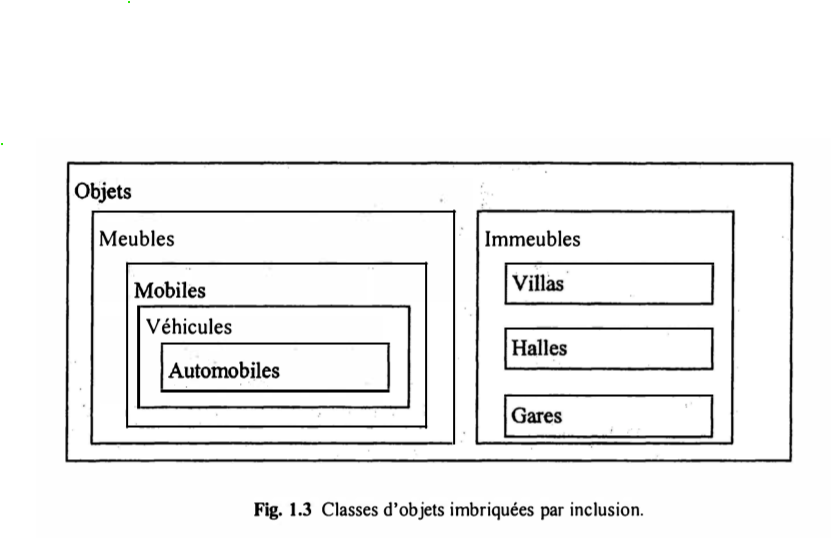
\includegraphics{1.3}
		\end{center}
	\end{figure}
\end{center}
Sự giảm dần từ cái tổng quát đến cái riêng này được diễn giải:\\
$\bullet$ en extension, như là một hiếm hoi dần dần của từng cá thể.\\
$\bullet$ en compréhension, như là một sự tích lũy các thuộc tính.\\
Ở giới hạn, một tập các thuộc tính thừa, thậm chí là mâu thuẫn, (chỉ) được thỏa mãn bởi 0 cá thể.
\end{document}